% !TEX program = xelatex
% Auto-generated by BeamerAgent — 2026-07-22
\documentclass[8pt,aspectratio=169]{beamer}

\usetheme[numbering=fraction,progressbar=frametitle]{metropolis}
\usepackage{fontspec}
\setmainfont{Times New Roman}
\usepackage{booktabs}
\usepackage{graphicx}
\graphicspath{{figures/}}
\usepackage{xcolor}
\usepackage{array}
\usepackage{colortbl}

\definecolor{mblue}{RGB}{0,82,147}
\definecolor{mgray}{RGB}{245,245,245}

\title{Thermodynamic Modeling: L-aspartic acid monosodium salt monohydrate}
\subtitle{NMC532 Leachate, Modifier 0.20 mol/kgw}
\author{MDPSA Pipeline}
\date{2026-07-22}
\institute{NRCan CC-NRCan-078}

\begin{document}

\maketitle

%% ── Slide 1: Model vs Experiment ─────────────────────────────────────────────
\begin{frame}{Model vs. Experiment}
  \begin{center}
    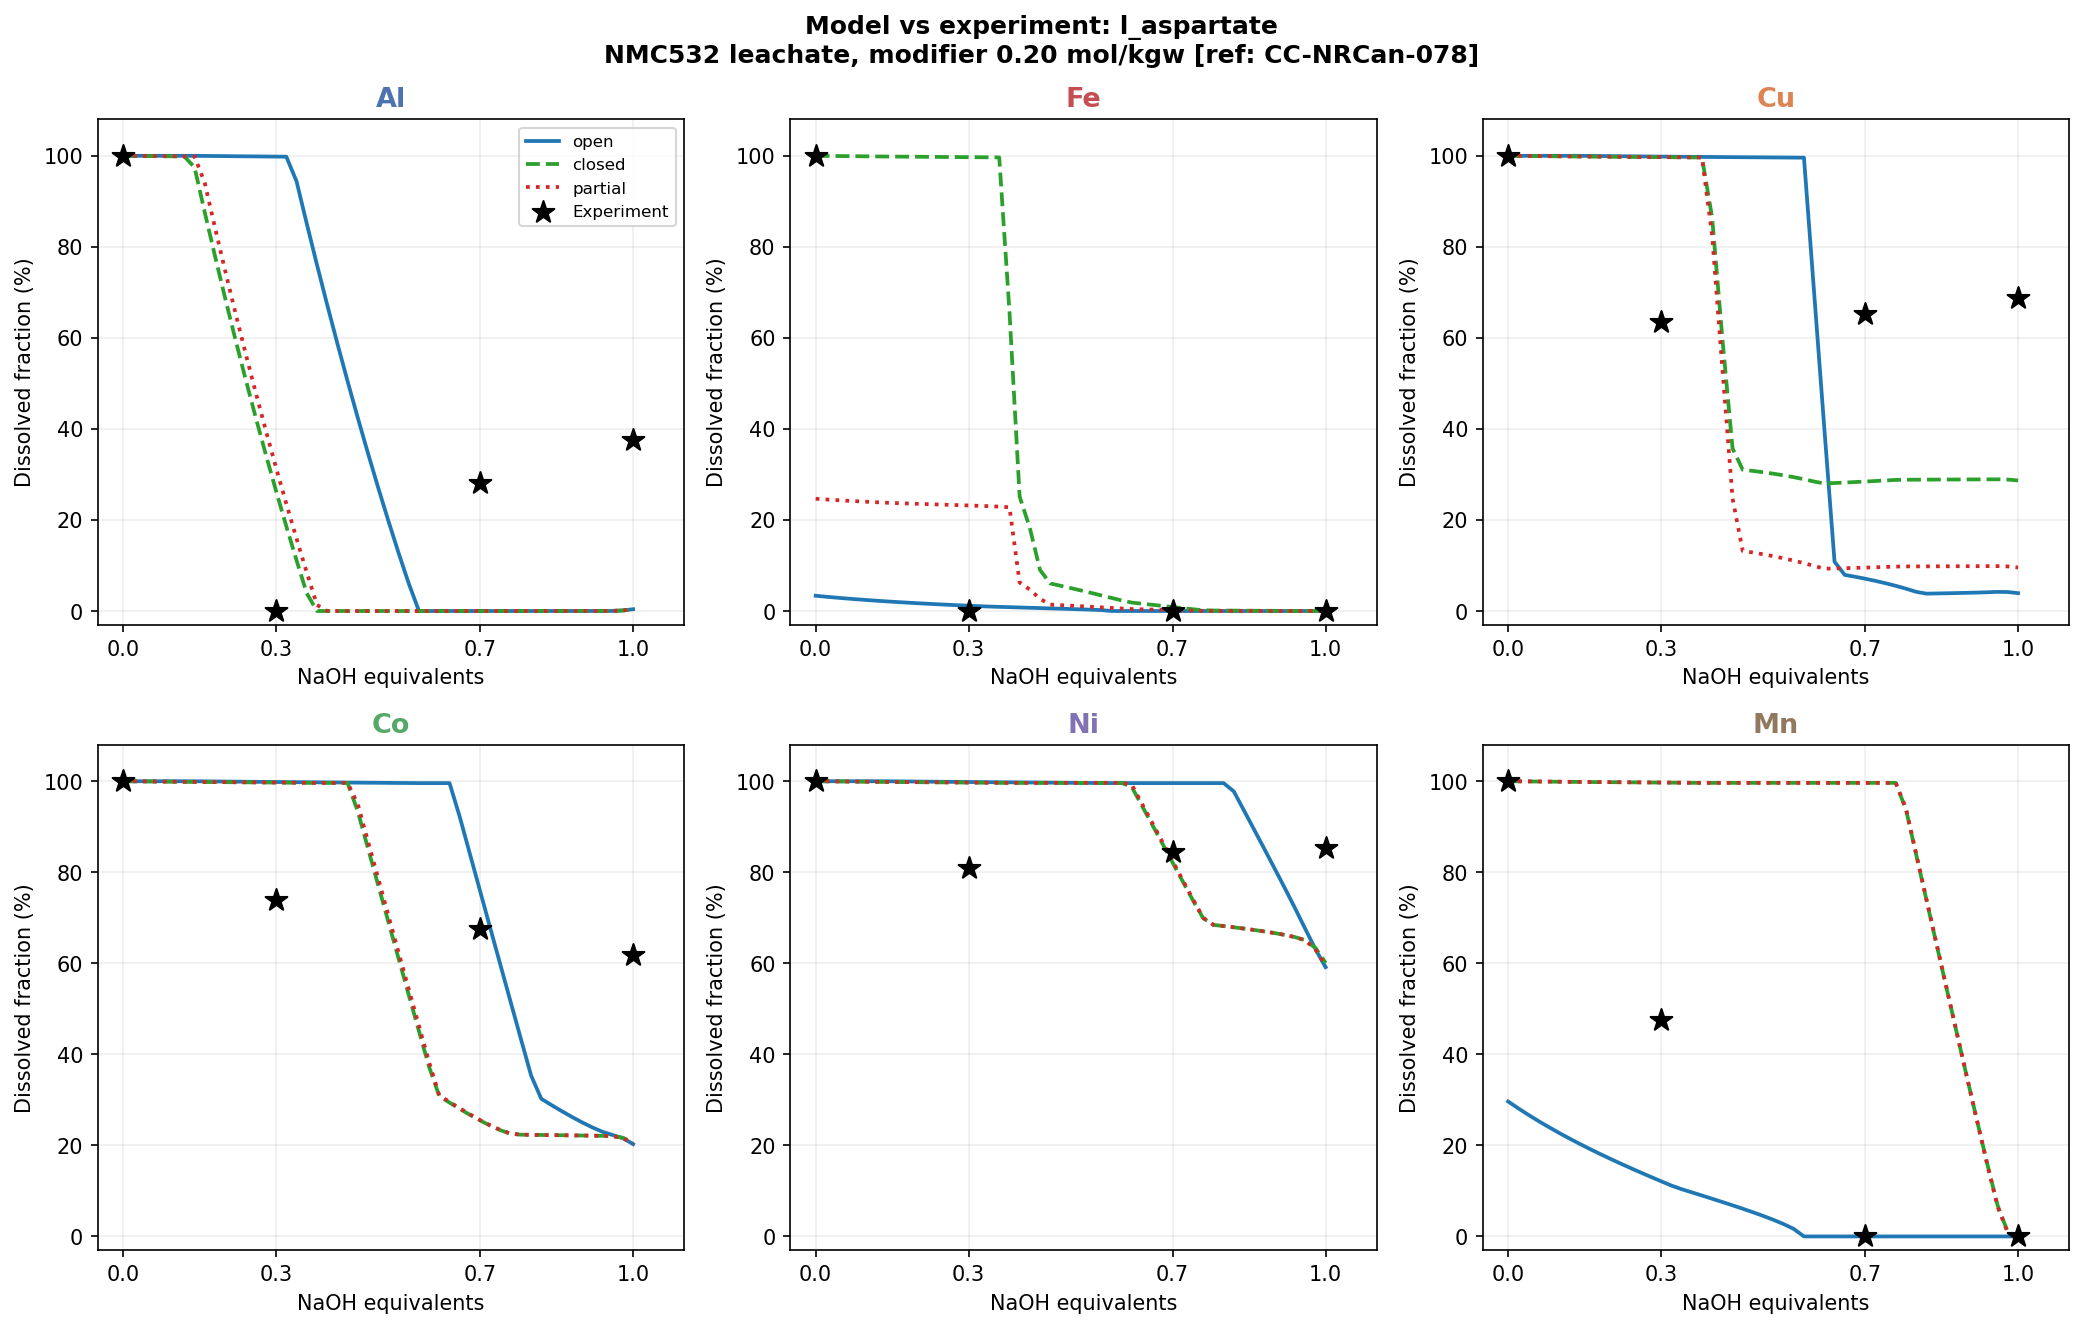
\includegraphics[width=0.92\textwidth,height=0.82\textheight,keepaspectratio]{l_aspartate_model_vs_exp.png}
  \end{center}
\end{frame}

%% ── Slide 2: Species Contributions ──────────────────────────────────────────
\begin{frame}{Species Contributions (Open System)}
  \begin{center}
    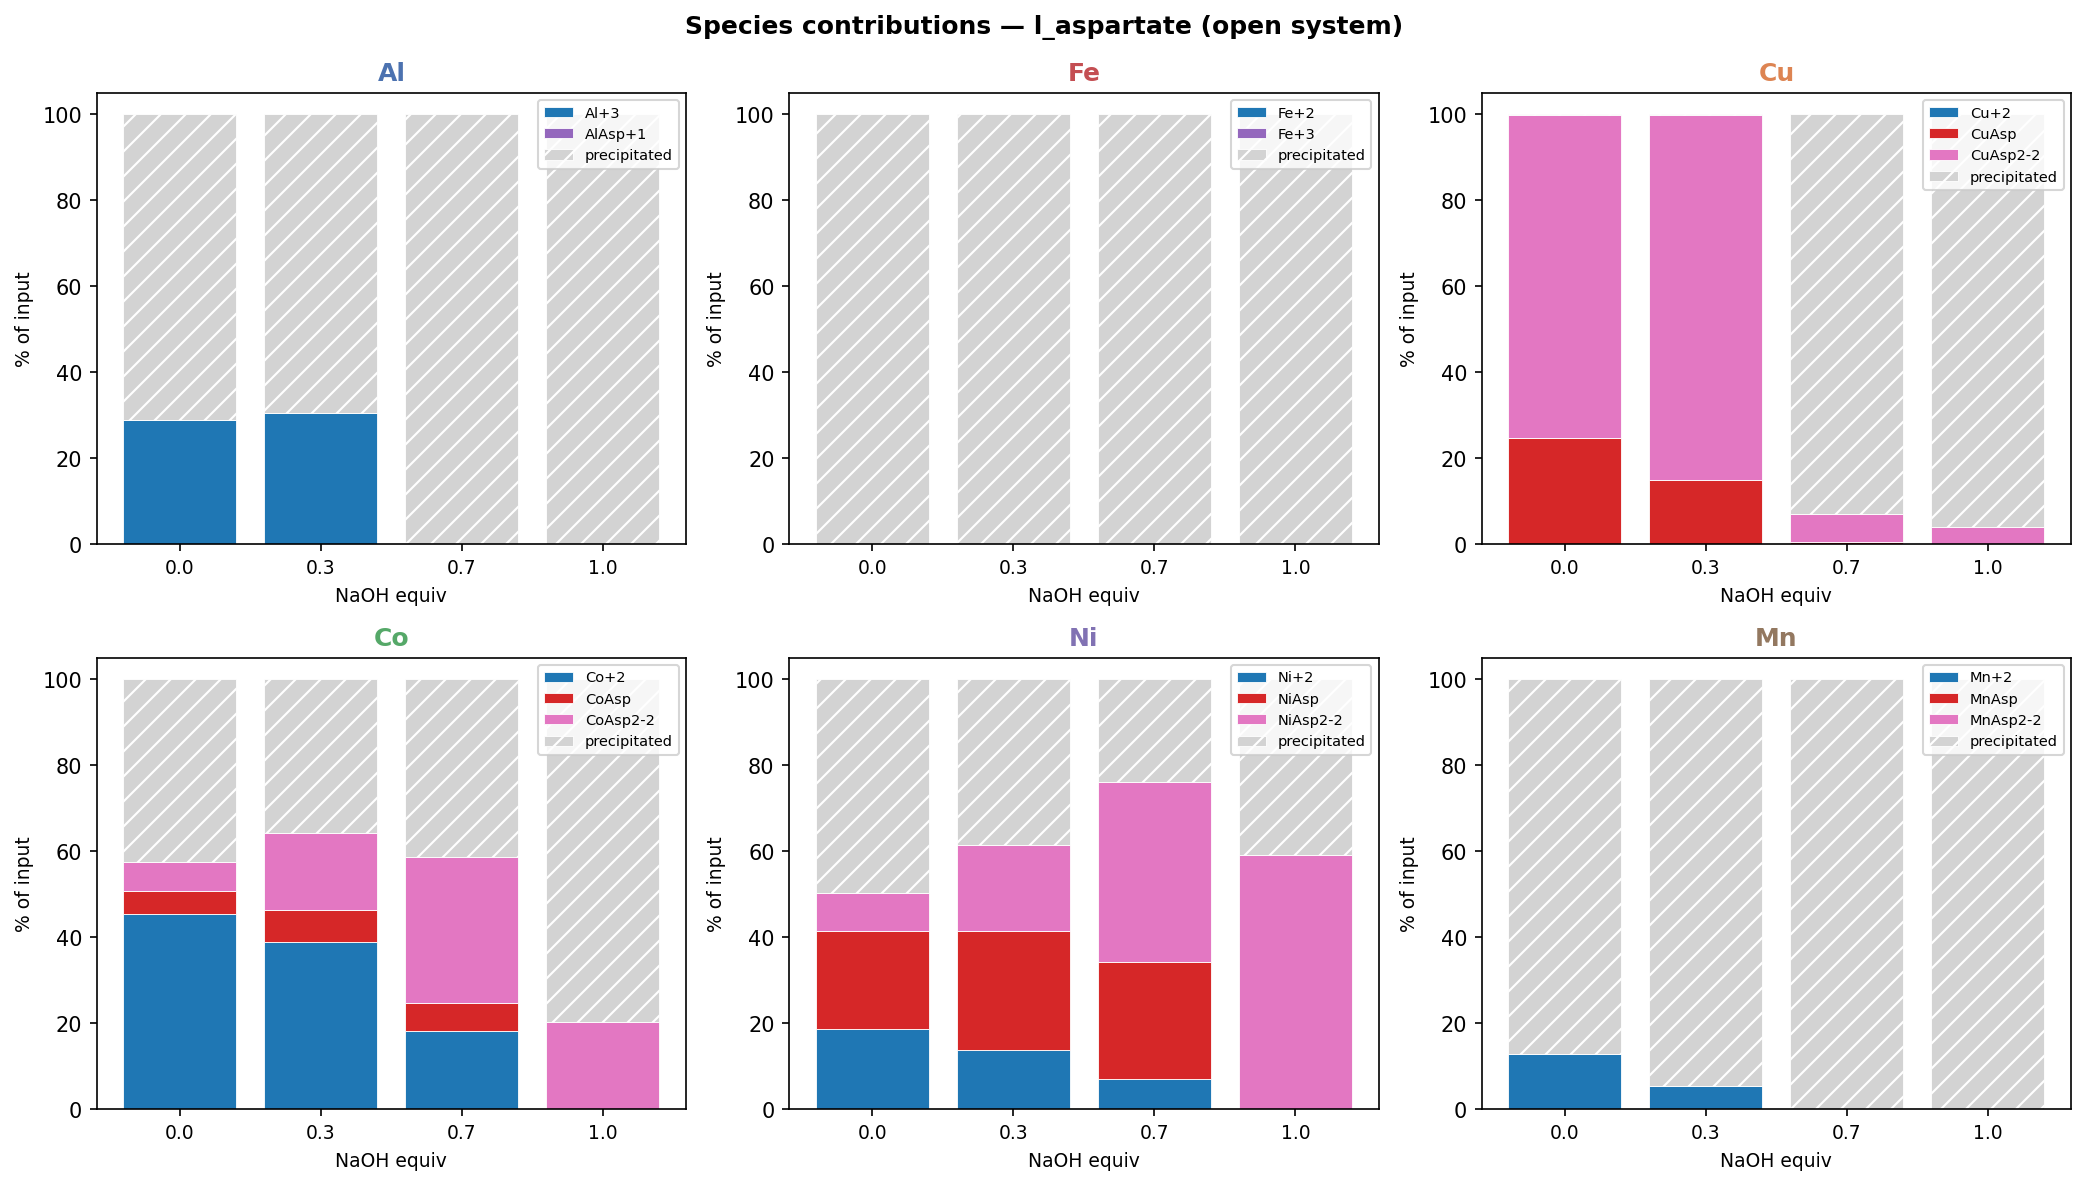
\includegraphics[width=0.92\textwidth,height=0.82\textheight,keepaspectratio]{l_aspartate_species_contribution.png}
  \end{center}
\end{frame}

%% ── Slide 3: Selectivity Scorecard ──────────────────────────────────────────
\begin{frame}{Selectivity Scorecard}
  \vspace{2pt}
  \begin{center}
  \small
  \setlength{\tabcolsep}{5pt}
  \renewcommand{\arraystretch}{1.3}
  \begin{tabular}{lllrrrr}
    \toprule
    \textbf{Metal} & \textbf{Role} & @ 0.3 eq & @ 1.0 eq & \textbf{RMSE (pp)} & \textbf{Verdict} \\
    \midrule
    Cu & Target & 100\% & 4\% & 47.2 & \textcolor{orange}{Partial} \\
    Co & Target & 100\% & 20\% & 24.8 & \textcolor{orange}{Partial} \\
    Ni & Target & 100\% & 59\% & 17.8 & \textcolor{green!60!black}{Protected} \\
    Mn & Target & 12\% & 0\% & 39.4 & \textcolor{red}{Lost} \\
    Al & Impurity & 100\% & 0\% & 55.1 & \textcolor{orange}{Partial} \\
    Fe & Impurity & 1\% & 0\% & 48.3 & \textcolor{green!60!black}{Removed} \\
    \bottomrule
  \end{tabular}
  \end{center}
  \vspace{4pt}
  \begin{beamercolorbox}[rounded=true, shadow=false, wd=\textwidth]{block body}
    \tiny
    RMSE: root-mean-square error in percentage points vs. experiment (CC-NRCan-078). \\
    Protected/Removed: model matches experiment at all comparison equiv points.
  \end{beamercolorbox}
\end{frame}

%% ── Slide 4: Thermodynamic Parameters ───────────────────────────────────────
\begin{frame}{Thermodynamic Parameters: L-aspartic acid monosodium salt monohydrate}
  \begin{columns}[T]
    \begin{column}{0.48\textwidth}
      \small
      \setlength{\tabcolsep}{6pt}
      \renewcommand{\arraystretch}{1.25}
      \begin{tabular}{lr}
        \toprule
        \textbf{Species} & \textbf{log K} \\
        \midrule
    CuAsp & 8.62 \\
    CuAsp2-2 & 14.00 \\
    CoAsp & 5.49 \\
    CoAsp2-2 & 10.50 \\
    NiAsp & 6.52 \\
    NiAsp2-2 & 11.00 \\
    MnAsp & 3.20 \\
    MnAsp2-2 & 2.50 \\
    AlAsp+1 & 3.50 \\
        \bottomrule
      \end{tabular}
    \end{column}
    \begin{column}{0.48\textwidth}
      \small
      \begin{itemize}
        \setlength{\itemsep}{4pt}
        \item Database: sit.dat (SIT activity model)
        \item Modifier dose: 0.20 mol/kgw
        \item Temperature: 25$^\circ$C, I = 0 (NIST reference)
        \item Equilibrium phases: Gibbsite, Ferrihydrite(am), \\
              Cu(OH)$_2$(s), Co(OH)$_2$(s), Ni(OH)$_2$(s), MnOOH
        \item Fe complexation suppressed (kinetic)
        \item Scenarios: open / closed / partial CO$_2$
      \end{itemize}
    \end{column}
  \end{columns}
  \vspace{4pt}
  \begin{beamercolorbox}[rounded=true, shadow=false, wd=\textwidth]{block body}
    \tiny
    Source: NIST Standard Reference Database 46 Version 8.0. Values adjusted for ionic-strength effects at leachate conditions.
  \end{beamercolorbox}
\end{frame}

\end{document}
